\chapter{Introduction}
\label{chap:intro}

Statistical machine translation (SMT) systems are trained using a large collection of translated
sentence pairs known as a parallel corpus. Common sources of parallel data include
parliament proceedings, books, and news articles.
For some language pairs, we have large amounts of this data. For example, the Canadian
Hansards are parliamentary proceedings that give us millions of words of
French/English parallel data \citep{Germann01}. Similarly, the proceedings of
European Union parliament are a source of parallel data for all of the languages
of its member states \citep{Koehn05}.
Outside of these government sources, we
also have large collections of parallel data from news agencies for some
language pairs, such as Chinese/English \citep{Ma05}.
However, for most language pairs, we have little to no data available.
In addition, even when parallel
data is available, it often does not match the domain of the data you wish to
translate, which hurts translation quality \citep{Munteanu05}.
Since the source of parallel corpora are institutions that want to disseminate
information in multiple languages, there will always be a bias in the genre of
the available data. Governments, news organizations, and international companies
are the most common sources of parallel data, giving us large amounts of text in
more formal domains, but leaving us with little in informal domains such as the
short, conversational text found on Twitter. 
Figure \ref{fig:europarl_twitter} gives some example parallel sentences from
Europarl as well as Twitter, showing the drastic difference in vocabulary and
syntax that can be found across domains.

\begin{figure*}[ht]
\begin{tabular}{|c|l|}
\hline
{\textbf Europarl} &\\
\hline
English & Please rise, then, for this minute' s silence. \\
Spanish & \tiny Invito a todos a que nos pongamos de pie para guardar un minuto de
silencio. \\
\hline
English & Madam President, on a point of order. \\
Spanish & Señora Presidenta, una cuestión de procedimiento. \\
\hline
\hline
\textbf{Twitter} &\\
\hline
English & can u listen to my song please? \\
Spanish & puede escuchar mi canci\'{o}n? \\
\hline
English & \tiny RT @celtics : Kobe Bryant surpassed Michael Jordan as the all-time NBA
\#AllStar scorer tonight.\\
Spanish & \tiny \#KobeBryant m\'{a}s puntos en \#AllStar games de todos los tiempos. :')\\
\hline
\end{tabular}
\caption{Parallel sentences from the European parliament and Twitter. The
Twitter data was selected from automatically mined data (see Chapter
\ref{chap:twitter}). While the Europarl sentences are well-formed and
grammatical, the sentences found on Twitter contain abbreviations, lack
punctuation, and contain markup and emoticons. In addition, the sentence pairs
we find on Twitter are not always exact translations, though we still may find
them to be useful as parallel data. We will explore this topic further in
Section \ref{sec:what_is_parallel}.}
\label{fig:europarl_twitter}
\end{figure*}

\adlbr{A point about motivation that doesn't quite come out here. Broadly, there
are two main customers for translation: those interested in disseminating information
in multiple languages (governments, news organizations, and international companies),
and those interested in assimilating information from multiple languages 
(intelligence agencies, travelers, consumers, researchers). The vast bulk of data
that we get is from the former, who generate it naturally in the course of their
day-to-day activities -- but their interests do not always coincide with
the needs of the latter, hence there is a mismatch between the data we have, and 
the data that we want. The easy to get data is what you get from web scraping.
However, to get data for the other customer base, you need to look for other signals
---evidence that people are talking about the same thing in multiple languages.}
\NoteJS{Added something in the first paragraph about this.}

The creation of new parallel corpora can be expensive, especially when bilingual
speakers are rare for the language pair of interest. \citet{Germann01a}
investigated the costs of collecting enough data to build Tamil/English SMT
system. They found that professionally translated data would cost $\$0.36$ per
word. \citet{Germann01a} and others \citep{Zaidan11} were able to reduce the
cost of creating parallel corpora by looking to non-professional translators,
but the cost is still around $\$0.10$ per word.
In order to acquire more parallel data without this cost,
researchers have looked to multilingual corpora which share some content across languages,
but are not directly translated. Such corpora are referred to as comparable
corpora, and examples include multilingual news feeds \citep{Munteanu05},
Wikipedia articles \citep{Adafre06,Smith10} (see Figure \ref{fig:wiki}), and the Web
\citep{Resnik99,Nie99,Chen00}. 

\begin{figure*}[ht]
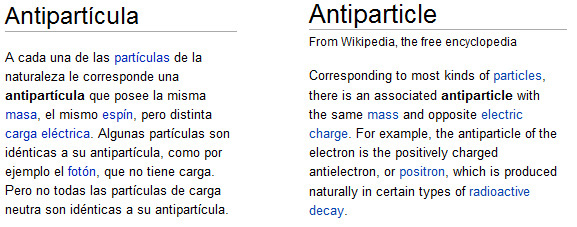
\includegraphics[width=\textwidth]{images/wiki.jpg}
\caption{An example of a Spanish/English document pair from Wikipedia.}
\label{fig:wiki}
\end{figure*}

The distinction between parallel and comparable corpora is not always clear.
Even corpora which are generally considered as parallel require some amount of
processing to find parallel sentences. 
A translator may chose to translate a compound sentence as two sentences, or
vice-versa, so naively assuming that sentences are aligned in order will not
work.
Also, there may be large insertions or deletions of sentences even in curated
sources of parallel data, such as the Canadian Hansards \citep{Gale93,Chen93}.
Sentence-aligning these corpora does not require existing parallel data or a
bilingual dictionary for the language pair of interest. Instead, the structure
of the documents and the lengths of the sentences are used to determine the
sentence alignment. When considering multilingual corpora which are less closely
related, additional signals must be used to
find parallel sentences. For corpora which are topic-aligned but not
directly translated, lexical information must be used to determine which
sentence pairs should be aligned \citep{Munteanu05}. When comparable corpora are
not topic-aligned, other signals such as URLs and hyperlinks are exploited to find plausible document
alignments \citep{Resnik03}.
\adlbr{This paragraph feels out of place.
Try reading the chapter, skipping this one completely. There's a pretty
nice flow from the previous to the next.}
\NoteJS{I moved it up and modified it to fit better.}

To give a better idea of the variety of comparable corpora, we will consider the
categorization of multilingual corpora given by \citet{Fung04a}:
\begin{enumerate}
\item Parallel corpus: A sentence-aligned corpus containing bilingual
translations of the same document. Curated parallel corpora fall in this
category.
\item Noisy parallel corpus: A corpus containing non-aligned sentences that are
nevertheless mostly bilingual translations of the same document. The Canadian Hansards,
Europarl, and most other parallel corpora are not strictly parallel until some
processing is done.
\item Comparable corpus: A corpus of non-aligned and non-translated documents
which are topic-aligned. Examples include multilingual social media discussions
linked by topic, and Wikipedia.
\item Quasi-comparable corpus: A multilingual corpus which is not
sentence-aligned, translated, or topic-aligned. This includes multilingual news
feeds and the Web.
\end{enumerate}
This is just one way of categorizing comparable corpora---there are concievably
many others. What is relevant for us is how the structure of different
comparable corpora allow us to find parallel data. For example, multilingual news feeds have
time stamps which help us align potentially parallel documents, while Wikipedia
contains links between articles on the same topic across languages. The methods
we use for mining parallel data will depend primarily on the signals available.

We will examine a representative set of comparable corpora: the Web, Twitter,
and Wikipedia; describe the different signals used to identify parallel data,
and demonstrate how extracted parallel data from these corpora improve SMT
performance across several language pairs and domains. First, we scale up
previous Web mining methods \citep{Resnik03} to several terabytes of data
(Chapter \ref{chap:data}). We
also present a novel mining approach for Twitter, making use of metadata unique
to the microblogging medium (Chapter \ref{chap:twitter}). Finally, we introduce a new sentence alignment
model for mining parallel data from Wikipedia which takes advantage of its
fine-grained topic alignment (Chapter \ref{chap:supervised}).
\NoteJS{I will come back to this ordering as I get to the other chapters.}

\section{What counts as parallel?}
\label{sec:what_is_parallel}
We are concerned with finding parallel data---bilingual sentence pairs
which convey the same meaning. Unfortunately, it is extremely difficult, if not
impossible, to determine whether or not two sentences in different languages
have the same meaning. One language may contain gender markings that the other
does not, or the connotation of a word may be difficult to express in another
language. Some examples of the ambiguity inherent in translation are explored by
\citet{Kay97}, one of which is shown in Figure \ref{fig:kay_ambig}.
Even ignoring the cross-lingual issues, comparing the meaning of two sentences
in the same language is still quite difficult---this is essentially the task of recognizing textual
entailment (RTE) \citep{Dagan10}.\footnote{RTE involves determining whether or
not one piece of text can be inferred from another.}
SMT evaluation metrics
\citep{Papineni02,Banerjee05,Snover06} must also address this problem when
comparing a hypothesis translation to a reference.

\begin{figure*}[ht]
\begin{tabular}{|c|l|}
\hline
French & Ils signeront le document pourvu que leur gouvernement accepte.\\
\hline
English & They will sign the document supplied that their government accepts. \\
English & They will sign the document provided that their government accepts. \\
English & They will sign the document on condition that their government accepts.\\
\hline
\end{tabular}
\caption{An example of a French sentence with multiple potential translations
into English taken from \citet{Kay97}.}
\label{fig:kay_ambig}
\end{figure*}

When evaluating methods for finding parallel data, we can either measure
intrinsic or extrinsic performance. Intrinsic evaluation directly measures the
quantity and quality of parallel data we extract, while extrinsic evaluation is
only concerned with how the new parallel data improves SMT performance.
In order to perform intrinsic evaluation, we need some criteria for determining whether or not a bilingual
sentence pair is parallel. This is easy if we use parallel data, but
it is preferable to evaluate our methods on the same corpora that we are
extracting data from. When designing the criteria for judging parallel
sentences, we focus on our extrinsic goal: improving SMT performance. If a sentence pair
is likely to improve performance when added to our SMT system's training data,
we would like to extract it. The details of our annotation criteria can be found
in Chapter \ref{chap:supervised}, but in all cases they are motivated by SMT
performance. To understand what will influence performance, we need to
understand modern SMT systems.

\section{Statistical Machine Translation}
While machine translation has been around in some form for many decades
\citep{Locke55}, statistical machine translation began with the work of
\citet{Brown88,Brown90,Brown93}. While SMT systems have evolved greatly since
then, they all share some key characteristics in how they use parallel data:
\adlbr{This feels a little opaque at this point:
either compress to lose unnecessary details, explain the difference in 
word-based, phrase-based, and syntax-based, give some examples, or move
this to a later point.}
\NoteJS{I compressed it. It doesn't seem necessary to go into details unless I
want to make a very specific point about how a system might handle a messy
parallel sentence pair.} 

\remove{
SMT systems have evolved since then, most notably moving from
word-based systems to phrase-based \citep{Koehn03}. Several newer systems have
been developed, focusing mostly on incorporating syntax into the translation
model \citep{Chiang05,Quirk05,Liu06,Galley06}.
}

\begin{enumerate}
\item A large collection of parallel sentences are used as training data.
\item For each parallel sentence, word-to-word correspondences are found. This
step is called word-alignment, and it is usually done with unsupervised methods
\citep{Brown93,Vogel96}.
\item Pairs of phrases, or other multi-word units, are extracted from the
word-aligned sentence pairs to form a translation model. Figure
\ref{fig:phrase_align} gives an example of an extracted phrase pair.
\item A language model is created from large amounts of monolingual data in the
``target'' language (the language which text is translated into). This includes
the target side of the parallel training data.
\end{enumerate}

\begin{figure*}[ht]
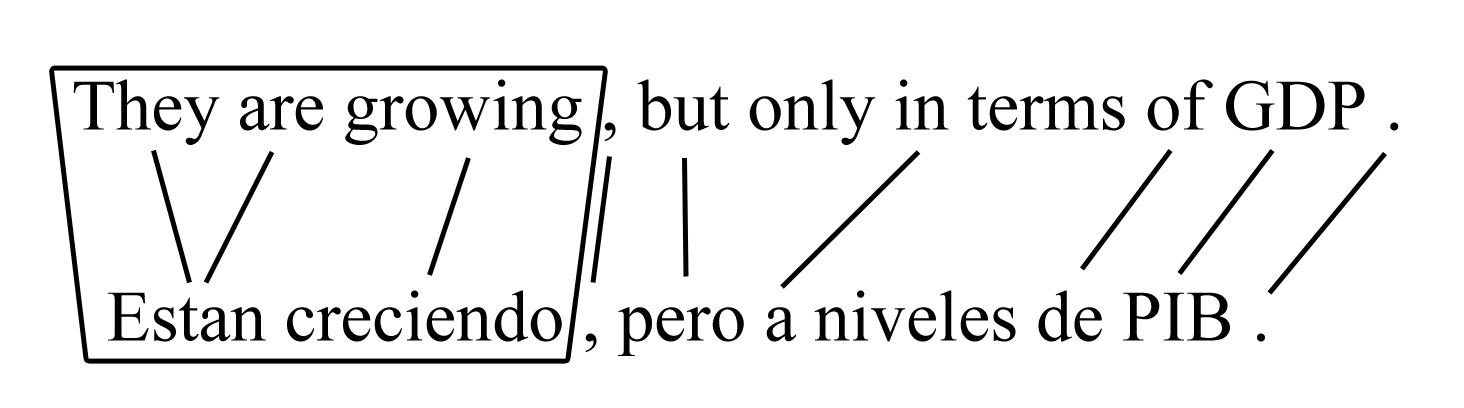
\includegraphics[width=\textwidth]{images/phrase_align.jpg}
\caption{A word-aligned sentence with an extracted phrase pair.}
\label{fig:phrase_align}
\end{figure*}

There are additional details in each model, but the main effects of adding new
parallel data are additional inputs to the translation and language models.

\section{Evaluation Pipeline}
Our evaluation setup is identical across chapters---we start with {\em initial}
data that includes some standard parallel and monolingual corpora commonly used for 
translation. We also have {\em extracted} parallel data that we find in a comparable
corpus. Table \ref{tab:exp_setup} describes how we use this data to measure SMT
improvements:

\begin{table}
\begin{center}
\begin{tabular}{|c||c|c|}
\hline
& Parallel & Monolingual \\
\hline
Baseline & Initial & Initial \\
\hline
Baseline + Monolingual & Initial & Initial + Extracted \\
\hline
Experimental & Initial + Extracted & Initial + Extracted \\
\hline
\end{tabular}
\end{center}
\label{tab:exp_setup}
\caption{Parallel and monolingual data used in our SMT experiments.}
\end{table}

In both the ``Baseline + Monolingual'' and ``Experimental'' conditions, we include the target side of
the extracted parallel sentences in the monolingual training data. We do this to
ensure that any increase in performance is coming from the parallel data. It
would be simple to add monolingual text from a comparable corpus to an SMT
system.

In all experiments, the BLEU metric \citep{Papineni02} is used to evaluate SMT
performance. It is the most commonly used evaluation metric, allowing us to
easily compare with other work.
The BLEU metric combines $n$-gram precision (the percentage of
$n$-grams in the hypothesis translation which are found in the reference) with a
brevity penalty. The exact formula is:
\begin{equation}
\exp(\min(1-\frac{r}{c},0) + \frac{1}{4}\sum^4_{n=1}\log p_n)
\end{equation}
where $r$ and $c$ are the reference and hypothesis lengths, and $p_n$ is the
$n$-gram precision.
The initial data, test sets, and other details vary by experiment.

\remove{
\section{Sentence Alignment}\adlbr{I agree that this probably does not fit here. The question is: what does? I think you might want to say something about prior art here, or otherwise fit in relevant parts of your lit review. Logically, a reader that has arrived at this point in your dissertation should understand the problem you're trying to solve at a high level, and might wonder what other approaches have been taken.}
In this section, we will describe our task and notation.
We will view both parallel corpora alignment and the extraction of parallel
sentences from comparable corpora as an alignment task. In either type of
alignment we are given a set of bilingual document pairs in {\em source} and {\em
target} languages. When performing parallel corpora alignment, these document
pairs will correspond to each other very strongly, while in the case of
comparable corpora, some these document pairs may contain no parallel sentences.
\citet{Munteanu05} take their document pairs from news stories published at
roughly the same time, while \citet{Adafre06,Smith10} use entries from
Wikipedia that are on the same topic (Figure \ref{fig:wiki} gives and example).
The task of finding comparable document pairs is not addressed in this work.

\begin{figure*}[ht]
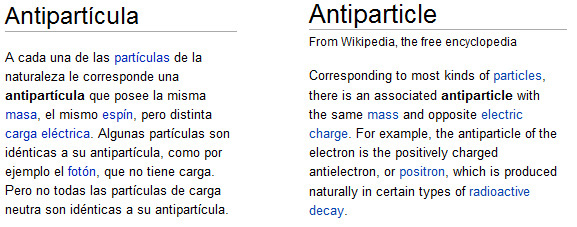
\includegraphics[width=\textwidth]{images/wiki.jpg}
\caption{An example of a Spanish/English document pair from Wikipedia.\adlbr{I think you want this example to appear in your comparable corpus section.}}
\label{fig:wiki}
\end{figure*}

Each document pair contains a sequence of source sentences (denoted by ${\bf
S}$) and target sentences (denoted by ${\bf T}$). Individual source and target
sentences are referred to by $S$ and $T$ respectively. Similarly, we refer to
the words within source and target sentences with the lowercase $s$ and $t$. We
borrow the notation of \citep{Och03} for describing alignments between sentences
as subsets of the Cartesian product of sentence positions. Sentence alignments
are referred to with the uppercase $A$, and word alignments with the lowercase
$a$.

The goal of sentence alignment is to identify which sentence pairs in the
bilingual document pairs are parallel. We view this as a retrieval task for
parallel sentence pairs, and so when annotated sentence alignments are present,
we can compute precision, recall, and F-measure.
}
